% Chapter 2

\chapter{Influence des Pratiques Individuelles sur la Durabilité en Ingénierie Logicielle}	%The main chapter title
\label{pratique-durabilite}
%%%%%%%%%%%%%%%%%%%%%%%%%%%%%%%%%%%%
Dans le domaine du génie logiciel, les pratiques individuelles des ingénieurs constituent un élément crucial de la recherche de durabilité. Ce chapitre explore l'influence de ces pratiques sur la durabilité des logiciels, examine les mesures pour un développement logiciel plus écologique et analyse l'impact du comportement des utilisateurs.


Le chapitre se décompose en trois sections distinctes, chacune apportant un éclairage unique sur la contribution des individus à des logiciels plus respectueux de l'environnement. La première section explore comment les choix et les actions des ingénieurs logiciels, en tant qu'individus, affectent la durabilité des logiciels qu'ils conçoivent et développent (Section~\ref{sec:pratiques-individuelles}). La deuxième section propose des mesures concrètes pour encourager un développement logiciel plus durable au niveau individuel (Section~\ref{sec:mesure-amelioration}). La dernière section examine le rôle crucial du comportement des utilisateurs dans la promotion de la durabilité des logiciels (Section~\ref{sec:comportement-utilisateurs}).

%%%%%%%%%%%%%%%%%%%%%%%%%%%%%%%%%%%%

\section{Impact des Pratiques Individuelles des Développeurs sur la Durabilité des Logiciels}
\label{sec:pratiques-individuelles}
%%%%%%%%%%%%%%%%%%%%%%%%%%%%%%%%%%%%

\subsection{Sensibiliser et renforcer les compétences}

Pour une adoption généralisée de pratiques d'ingénierie logicielle écologiques, des avancées techniques ne suffisent pas. Il est également nécessaire de sensibiliser les développeurs et de leur fournir les connaissances nécessaires.


Le manque de compréhension des développeurs sur l'impact environnemental des logiciels est un problème avéré. L'article~\cite{EmpiricalStudy} évoque bien ce point : \emph{« I care about memory usage, CPU usage, like I understand those. [...] I don’t have the same intuition about energy. »} Pour combler ce manque, des initiatives éducatives sont essentielles. Elles permettront aux développeurs d'acquérir des connaissances et des compétences nécessaires pour contribuer efficacement au développement de logiciels verts.


La mesure des logiciels verts joue un rôle clé dans cette démarche. Selon l'article~\cite{GreenMeasurementStructure}, \emph{« Green software measurement aims to provide and offer software practitioners and stakeholders a mechanism to measure the green compliance of software products, which will help them ensure their software's naturalness in their organizations. »} En établissant des mesures mesurables et des références quantifiables, les développeurs peuvent évaluer l'impact environnemental de leurs logiciels et prendre des décisions fondées sur des données en vue d'une plus grande durabilité.


Cependant, il est important de reconnaître que la connaissance et la sensibilisation ne reposent pas uniquement sur l'expertise technique. L'article~\cite{SustainabilityAwarenessFramework} met en avant l'importance des connaissances du facilitateur pour l'efficacité des ateliers sur la durabilité. Plus précisément, il souligne que \emph{« The quality of the sustainability workshops, their outcomes, and the mappings between the identified sustainability effects and the backlog items are influenced by the knowledge, experience, and understanding of the first author who conducted. »} Le besoin d'une sensibilisation accrue à tous les niveaux du développement logiciel devient crucial. En effet, la création d'un environnement collaboratif où chaque acteur, des développeurs aux gestionnaires et aux parties prenantes, peut apprendre et partager ses connaissances est essentielle pour construire un avenir durable. Cette collaboration permet à chacun d'apporter sa contribution unique et de maximiser l'impact positif sur l'environnement.


De plus, la citation de~\cite{SustainabilityAwarenessFramework} met en exergue la subjectivité inhérente aux perceptions de la durabilité : \emph{« The results also depend on the experience of the first author who led the workshops, and also on the perception of sustainability by the other workshop participants. »} Des dialogues et des discussions inclusives sont donc nécessaires pour combler le fossé entre les différentes perspectives et créer une compréhension commune de ce que signifie développer des logiciels de manière durable.


La sensibilisation et le renforcement des compétences sont des éléments clés pour une adoption réussie de pratiques d'ingénierie logicielle écologique. Des initiatives éducatives, des mesures de logiciels verts et une sensibilisation à tous les niveaux sont essentiels pour doter les développeurs des outils et de la compréhension nécessaires pour contribuer à un avenir numérique plus durable.

% Sensibilisation et connaissance des développeurs
%~\cite{EmpiricalStudy} "I care about memory usage, CPU usage, like I understand those. [...] I don’t have the same intuition about energy."
%~\cite{GreenMeasurementStructure} "Green software measurement aims to provide and offer software practitioners and stakeholders a mechanism to measure the green compliance of software products, which will help them ensure their software's naturalness in their organizations."
%~\cite{SustainabilityAwarenessFramework} "The quality of the sustainability workshops, their outcomes, and the mappings between the identified sustainability effects and the backlog items are influenced by the knowledge, experience, and understanding of the first author who conducted."
%~\cite{SustainabilityAwarenessFramework} "The results also depend on the experience of the first author who led the workshops, and also on the perception of sustainability by the other workshop participants."

\subsection{Équilibrer les priorités et négocier des compromis}

La recherche d'un développement logiciel durable implique souvent de faire des compromis complexes et d'établir des priorités entre des objectifs concurrents.

\paragraph{Performance contre consommation d'énergie :}
L'article~\cite{EmpiricalStudy} abonde dans ce sens, soulignant que les compromis entre performances et consommation d'énergie sont inévitables : \emph{« Only when meeting performance goals becomes egregious in terms of power, then we negotiate a compromise that balances performance and power consumption. »} Cette citation met en lumière l'épineuse question de l'équilibre entre performances et efficacité énergétique. En effet, la maximisation simultanée de ces deux aspects s'avère souvent impossible, ce qui implique des compromis nécessairement adaptés aux exigences spécifiques de chaque projet et aux priorités des parties prenantes.

\paragraph{Impacts de premier ordre contre impacts de second ordre :}
Au-delà des effets de premier ordre, il est crucial de considérer les ramifications indirectes et en cascade, que l'on appelle effets de deuxième et troisième ordre. La citation de~\cite{SafetySecuritySustainability} résume parfaitement cette nécessité : \emph{« Software engineers can considerably improve civilization’s sustainability by taking into account not just the first-order impacts of software systems, but also their second- and third-order impacts. »} En d'autres termes, une approche holistique s'impose. Se focaliser uniquement sur la consommation d'énergie immédiate des logiciels ne suffit pas. Il est essentiel d'évaluer leurs implications sociétales et environnementales plus larges. C'est en adoptant une vision globale que nous pourrons véritablement contribuer à un développement logiciel durable.

\paragraph{Négocier des compromis :}
C'est souvent aux ingénieurs logiciels, en collaboration avec d'autres parties prenantes, qu'incombe la responsabilité de trouver un équilibre entre ces priorités concurrentes. L'article~\cite{SafetySecuritySustainability} met en lumière cet enjeu : \emph{« The challenge of incorporating this conflict into software engineering is an issue of requirements prioritization, which is usually handled by negotiation between system stakeholders. »} Pour relever ce défi, une communication ouverte et une prise de décision collaborative s'avèrent essentielles. Dès le début du processus de développement logiciel, il est crucial d'intégrer les réflexions sur la durabilité. Cela ne peut se faire qu'en favorisant un dialogue constructif entre tous les acteurs impliqués.


La recherche d'un développement logiciel durable implique de naviguer dans un paysage complexe de priorités concurrentes et de compromis délicats. La prise en compte des impacts de premier et de second ordre, ainsi que la négociation transparente entre les parties prenantes, sont essentielles pour garantir que les logiciels contribuent à un avenir numérique plus durable.

% Priorités et compromis
%~\cite{EmpiricalStudy} "Only when meeting performance goals becomes egregious in terms of power, then we negotiate a compromise that balances performance and power consumption."
%~\cite{SafetySecuritySustainability} "Software engineers can considerably improve civilization’s sustainability by taking into account not just the first-order impacts of software systems, but also their second- and third-order impacts."
%~\cite{SafetySecuritySustainability} "The challenge of incorporating this conflict into software engineering is an issue of requirements prioritization, which is usually handled by negotiation between system stakeholders."

\subsection{Bien-être des développeurs et processus de prise de décision}

Bien que l'adoption de pratiques d'ingénierie logicielle écologiques soit essentielle pour la durabilité environnementale, il est également crucial de prendre en compte le bien-être des développeurs et l'impact potentiel sur leurs processus de prise de décision.


Des études, comme celle de~\cite{EmpiricalStudy}, indiquent que les préoccupations énergétiques peuvent influencer l'écriture du code par les développeurs. La citation \emph{« Energy concerns influence how practitioners write new code. »} souligne le potentiel d'augmentation de la charge cognitive liée à la responsabilité supplémentaire de l'optimisation énergétique. En d'autres termes, l'intégration de l'efficacité énergétique dans le développement logiciel peut s'avérer cognitivement exigeante. Les développeurs doivent désormais jongler entre les exigences fonctionnelles du logiciel et la recherche de solutions économes en énergie.


L'article~\cite{SustainableEngNeglectedPerspective} rappelle les limites de la mémoire de travail humaine. Deux citations illustrent ce point: \emph{« The capacity of the human working memory and the amount of cognitive load it can process (i.e., cognitive bandwidth) are closely related »} et \emph{« overloading a human’s 'limited' working memory inhibits his learning ability and problem-solving skills. »} En conséquence, il est crucial d'évaluer l'impact potentiel des pratiques de développement logiciel durable sur la charge cognitive des développeurs. L'objectif est de les mettre en œuvre de manière à soutenir, et non à entraver, leurs capacités cognitives.


L'étude publiée dans~\cite{SustainableEngNeglectedPerspective} met en évidence le lien entre le manque de contrôle et l'épuisement professionnel : \emph{« A lack of independence or control at work and prolonged pressure increases the risks of burnout in software engineers. »} Elle souligne également les conséquences potentielles d'un compromis sur le bien-être des développeurs : \emph{« Developing software under such circumstances not only affects the mental health of the engineers but also compromises the quality of the produced software. »} Cette affirmation démontre l'interconnexion entre le bien-être des développeurs, la qualité des logiciels et, en fin de compte, le succès des initiatives d'ingénierie logicielle écologique.


Le bien-être des développeurs est intrinsèquement lié à la qualité des logiciels et au succès des initiatives d'ingénierie logicielle écologique. Il est donc crucial de concevoir et de mettre en œuvre ces pratiques de manière à minimiser la charge cognitive, à offrir un sentiment de contrôle et à soutenir le bien-être des développeurs. En trouvant un équilibre entre les exigences environnementales et les besoins humains, nous pouvons garantir un avenir durable et épanouissant pour le développement de logiciels.

% Bien-être des développeurs et prise de décision
%~\cite{EmpiricalStudy} "Energy concerns influence how practitioners write new code."
%~\cite{SustainableEngNeglectedPerspective} "The capacity of the human working memory and the amount of cognitive load it can process (i.e., cognitive bandwidth) are closely related."
%~\cite{SustainableEngNeglectedPerspective} "Overloading a human’s 'limited' working memory inhibits his learning ability and problem-solving skills."
%~\cite{SustainableEngNeglectedPerspective} "A lack of independence or control at work and prolonged pressure increases the risks of burnout in software engineers."
%~\cite{SustainableEngNeglectedPerspective} "Developing software under such circumstances not only affects the mental health of the engineers but also compromises the quality of the produced software."

\subsection{Comportement et sensibilisation des utilisateurs}

Pour atteindre les objectifs de l'ingénierie logicielle verte, il est nécessaire de dépasser le processus de développement et de favoriser la participation active des utilisateurs.


Saisir l'écart entre les intentions déclarées et le changement de comportement réel est crucial. La citation de~\cite{ImpactGreenFeedback} l'illustre parfaitement : \emph{« In contrast, users who stated to change behavior when doing less important tasks, did not translate into power reductions. »} En clair, cette citation met en lumière un décalage possible entre la sensibilisation des utilisateurs et l'adoption durable de nouveaux comportements. En d'autres termes, fournir des informations ne suffit pas nécessairement à garantir un changement à long terme.


Nuançons notre propos. Si l'écart entre intentions et actions est réel, les recherches soulignent aussi l'impact positif des commentaires écologiques sur la sensibilisation des utilisateurs et leur adoption de pratiques économes en énergie. L'étude~\cite{ImpactGreenFeedback} le confirme : \emph{« We find that green feedback helps in raising awareness about software energy, and on the willingness of users to apply energy-efficient changes. »} Fournir aux utilisateurs des informations claires et exploitables sur l'impact environnemental de leur utilisation de logiciels peut être un outil puissant pour encourager un comportement durable.


L'intention ne suffit pas toujours. Même si les utilisateurs souhaitent s'engager dans le développement durable, ils peuvent manquer des connaissances et des outils nécessaires pour le faire de manière efficace. L'article~\cite{ImpactGreenFeedback} le souligne : \emph{« Participants also miss the tools and the knowledge of what to do to change their behavior, even if they want to. »} Des initiatives éducatives sont cruciales pour combler ce manque. Elles doivent outiller les utilisateurs et leur fournir les compétences et ressources pratiques pour faire des choix éclairés quant à leur utilisation des logiciels. C'est la clé pour construire un avenir plus durable.


Le comportement et la sensibilisation des utilisateurs sont des éléments clés pour une adoption réussie des pratiques d'ingénierie logicielle écologique. Un effort concerté pour fournir des commentaires clairs, des outils pratiques et des initiatives éducatives est essentiel pour encourager une utilisation responsable des logiciels et contribuer à un avenir numérique plus durable.

% Comportement et sensibilisation des utilisateurs
%~\cite{ImpactGreenFeedback} "In contrast, users who stated to change behavior when doing less important tasks, did not translate into power reductions."
%~\cite{ImpactGreenFeedback} "We find that green feedback helps in raising awareness about software energy, and on the willingness of users to apply energy-efficient changes."
%~\cite{ImpactGreenFeedback} "Participants also miss the tools and the knowledge of what to do to change their behavior, even if they want to."

\subsection{Mesure et évaluation}

La mesure des logiciels verts joue un rôle crucial dans l'évaluation de l'efficacité des pratiques d'ingénierie logicielle verte et dans la démonstration des progrès vers les objectifs de durabilité.


L'article~\cite{GreenMeasurementStructure} définit clairement l'ambition de la mesure logicielle verte : \emph{« Green software measurement aims to provide and offer software practitioners and stakeholders a mechanism to measure the green compliance of software products, which will help them ensure their software's naturalness in their organizations. »} Il s'agit de fournir aux développeurs et aux parties prenantes un outil pour mesurer la conformité écologique des produits logiciels. Cela leur permet de garantir l'intégration naturelle de l'aspect environnemental dans leurs organisations. L'établissement de mesures concrètes et de références quantifiables est crucial. Cela permet d'évaluer objectivement l'impact environnemental des logiciels et de suivre les progrès réalisés au fil du temps.


L'ambition du logiciel vert ne se limite pas à la seule dimension environnementale. L'ouvrage~\cite{GreenMeasurementStructure} insiste sur la nécessité d'une approche holistique : \emph{« We can accomplish green software product by applying the complete three elements of sustainability as mentioned in the previous section of this paper: social, economic, and environmental. »} En d'autres termes, il est crucial de mesurer et d'évaluer les logiciels selon les trois piliers de la durabilité : social, économique et environnemental. Tout en permettant de garantir que les progrès vers un avenir durable soient équitables et complets, ne laissant personne de côté et ne sacrifiant aucun aspect au profit d'un autre.


Le choix des bons paramètres est crucial pour une évaluation efficace. L'article~\cite{GreenMeasurementStructure} le rappelle : \emph{« The required measurements of sustainable features define for evaluating the target. It comprises measures that influence green products [...]. If the measurements are good in sustainability dimensions, delivered product would also have a high level of green. »} Des mesures bien choisies et percutantes permettent de capturer l'essence du développement de logiciels verts et d'obtenir des informations précieuses. La communauté du développement de logiciels peut ainsi évaluer l'efficacité de ses efforts et identifier les domaines à améliorer pour progresser vers un avenir plus durable.


Pour couronner le tout, une méthodologie de mesure structurée s'avère indispensable. L'article~\cite{GreenMeasurementStructure} propose un processus de décomposition pertinent : \emph{« Green software elements are decomposed into measurements and sub measurements. Then, the sub measurement is broken down to a further level of decomposition that associate with direct assessment metrics. »} Cette approche hiérarchique permet d'évaluer systématiquement tous les aspects d'un logiciel écologique. Elle offre une compréhension globale du profil de durabilité du produit, ne laissant aucun élément dans l'ombre.


La mesure et l'évaluation sont des éléments clés pour une adoption réussie des pratiques d'ingénierie logicielle écologique. Une approche holistique, axée sur la sélection de paramètres pertinents et une méthodologie structurée, est essentielle pour fournir des informations précises et exploitables sur l'impact environnemental des logiciels.

% Mesure et évaluation
%~\cite{GreenMeasurementStructure} "Green software measurement aims to provide and offer software practitioners and stakeholders a mechanism to measure the green compliance of software products, which will help them ensure their software's naturalness in their organizations."
%~\cite{GreenMeasurementStructure} "We can accomplish green software product by applying the complete three elements of sustainability as mentioned in the previous section of this paper: social, economic, and environmental."
%~\cite{GreenMeasurementStructure} "The required measurements of sustainable features define for evaluating the target. It comprises measures that influence green products, as mentioned in [33]. If the measurements are good in sustainability dimensions, delivered product would also have a high level of green."
%~\cite{GreenMeasurementStructure} "Green software elements are decomposed into measurements and sub measurements. Then, the sub measurement is broken down to a further level of decomposition that associate with direct assessment metrics."

\subsection{Influences sociétales et systémiques}

La poursuite de l'ingénierie logicielle verte va au-delà des solutions techniques et aborde les problèmes sociétaux et systémiques plus larges qui contribuent aux défis environnementaux.


La citation de~\cite{SafetySecuritySustainability} attire notre attention sur les conséquences inattendues de nos choix, individuels et sociétaux : \emph{« It isn’t civilization’s intention to harm the Earth, but the collective sum of our individual actions, which often favor local convenience over global responsibility, added to the effects of the societal structures we’ve created lead to negative consequences for our environment. »} Si l'intention de nuire à la planète n'est pas préméditée, nos actions individuelles, privilégiant souvent la commodité locale au détriment de la responsabilité globale, s'additionnent et, combinées aux effets des structures sociétales que nous avons créées, génèrent des conséquences néfastes pour l'environnement. Ce constat appelle à un changement de perspective. Il est crucial de dépasser la simple recherche de la commodité individuelle et d'adopter un sentiment de responsabilité collective envers le bien-être environnemental.


L'atteinte de la durabilité exige une transformation systémique profonde. L'article~\cite{SafetySecuritySustainability} l'affirme clairement : \emph{« If our civilization is to transition to sustainability, many sectors of society will need to rethink their modes of operation. »} L'ingénierie logicielle verte ne peut être une solution isolée. Elle s'inscrit comme une pièce d'un puzzle plus vaste, nécessitant une collaboration et des efforts coordonnés entre les différentes parties prenantes.


L'étude de~\cite{SafetySecuritySustainability} introduit un concept novateur : la \emph{« explicit stakeholder for environmental sustainability. »} Cette idée incite à la réflexion et suggère que des solutions durables pourraient exiger une formalisation de la responsabilité environnementale au sein des structures organisationnelles et des processus décisionnels.


En reconnaissant l'imbrication des facteurs sociétaux et systémiques, en encourageant l'action collective et en explorant des solutions innovantes comme celle proposée par~\cite{SafetySecuritySustainability}, la communauté du développement de logiciels peut jouer un rôle crucial dans la construction d'un avenir plus durable.


Dans ce contexte élargi, l'ingénierie logicielle verte devient bien plus qu'un simple défi technique ; elle se révèle être un véritable catalyseur de changement sociétal positif.

% Influences sociétales et systémiques
%~\cite{SafetySecuritySustainability} "It isn’t civilization’s intention to harm the Earth, but the collective sum of our individual actions, which often favor local convenience over global responsibility, added to the effects of the societal structures we’ve created lead to negative consequences for our environment."
%~\cite{SafetySecuritySustainability} "If our civilization is to transition to sustainability, many sectors of society will need to rethink their modes of operation."
%~\cite{SafetySecuritySustainability} "Perhaps the solution requires an explicit stakeholder for environmental sustainability."

\subsection{Définition du logiciel durable}

Le concept de logiciel durable ne se limite pas à la simple réduction de l'empreinte environnementale. Il embrasse une vision holistique qui intègre l'influence du logiciel sur divers aspects, comme le souligne l'article~\cite{GreenMeasurementStructure} :

\begin{quote}
    
    \emph{« Sustainable software is related to its influence on the economy, society, people, and the environment. It is the consequence of minor upgrades, delivery, and use of software and positively impacts sustainability. »}
    
\end{quote}


Cette définition met en lumière le fait que les logiciels durables ne se contentent pas de minimiser les impacts environnementaux négatifs, mais qu'ils génèrent également des avantages concrets dans plusieurs dimensions :

\begin{itemize}
    \item \textbf{Économique :} Les pratiques de développement durable de logiciels peuvent contribuer à des économies de coûts, à l'optimisation des ressources et à la création d'emplois.
    \item \textbf{Social :} Elles peuvent promouvoir un accès équitable à la technologie, améliorer l'expérience utilisateur et participer à une société plus inclusive.
    \item \textbf{Environnemental :} Aspect le plus reconnu, les logiciels durables minimisent la consommation d'énergie, réduisent la production de déchets électroniques et contribuent à un environnement plus sain.
\end{itemize}


Un logiciel durable ne se résume pas à un produit statique, mais plutôt à l'aboutissement d'un processus de développement réfléchi qui intègre, dès sa conception, l'ensemble du cycle de vie du logiciel et ses implications sociétales et environnementales. Il est le fruit d'une amélioration continue et d'efforts constants pour créer des solutions logicielles qui ne se limitent pas à leur fonctionnalité, mais qui se distinguent par leur responsabilité et leur contribution positive au monde qui nous entoure.

% Définition du logiciel durable
%~\cite{GreenMeasurementStructure} "Sustainable software is related to its influence on the economy, society, people, and the environment. It is the consequence of minor upgrades, delivery, and use of software and positively impacts sustainability."

\subsection{Charge cognitive}

L'affirmation de~\cite{SustainableEngNeglectedPerspective} stipulant que \emph{« Cognitive load is considered a waste in SE »} soulève des inquiétudes. En effet, elle implique une méconnaissance du bien-être des ingénieurs logiciels et une interprétation erronée du concept de charge cognitive dans ce domaine.

\paragraph{Comprendre l'impact de la charge cognitive sur les développeurs}
Prenons l'exemple de la multiplication mentale, proposé dans l'ouvrage "La Charge Cognitive : Théorie et Applications"~\cite{ChargeCognitive} : 

\begin{enumerate}
    \item \emph{« effectuer mentalement la multiplication $7 \times 6 = ?$ est très facile »}
    \item \emph{« $7 \times 42 = ?$ nécessite un effort pour retrouver en mémoire les informations nécessaires au calcul »}
    \item \emph{« $294 \times 7 896 = ?$ est extrêmement compliqué à calculer de tête, très long, et sans doute impossible à réaliser pour la plupart des individus. »}
\end{enumerate}


Cet exemple illustre parfaitement l'impact de la charge cognitive sur les tâches quotidiennes. La complexité de la tâche, la quantité d'informations à traiter et la familiarité avec la tâche sont autant de facteurs qui influencent la charge cognitive et, par conséquent, la performance et le bien-être des individus.


Dans le domaine du développement logiciel, la charge cognitive peut être particulièrement élevée en raison de la complexité des tâches, de la quantité d'informations à traiter et du rythme effréné du travail. Une charge cognitive excessive peut alors engendrer du stress, de l'épuisement professionnel et une baisse de la productivité, nuisant ainsi au bien-être des ingénieurs logiciels.

\paragraph{Démystifier la notion de charge cognitive}
Qualifier la charge cognitive de \emph{« waste »} suggère qu'elle est intrinsèquement négative et doit être systématiquement évitée. Or, il est important de noter que la charge cognitive n'est pas intrinsèquement mauvaise. En réalité, un certain niveau de charge cognitive est nécessaire pour apprendre, résoudre des problèmes et accomplir des tâches complexes. L'enjeu réside dans la gestion efficace de la charge cognitive afin qu'elle demeure dans une zone optimale et ne devienne pas excessive pour les développeurs.


Reprenons l'exemple des multiplications citées précédemment. Si la tâche $7 \times 6 = ?$ ne présente que peu de challenge et ne mobilise que peu de ressources cognitives, elle ne permet pas non plus d'apprentissage ou de développement significatif. En revanche, la tâche $294 \times 7 896 = ?$, bien que complexe, peut être source d'apprentissage et de satisfaction si elle est abordée de manière adéquate. L'enjeu est donc de trouver un équilibre entre des tâches trop simples et des tâches trop complexes, afin de maintenir la charge cognitive dans une zone optimale pour l'apprentissage et la performance.


Il est important de noter que la charge cognitive est un concept subjectif. Ce qui peut être une charge cognitive excessive pour un individu peut ne pas l'être pour un autre. De même, la charge cognitive peut varier en fonction du contexte et des conditions de travail.


La charge cognitive est un élément important à prendre en compte dans le domaine du développement logiciel. En comprenant les facteurs qui influencent la charge cognitive et en adoptant des pratiques pour la gérer efficacement, il est possible d'améliorer le bien-être et la performance des développeurs logiciels.

% Charge cognitive
%~\cite{SustainableEngNeglectedPerspective} "Cognitive load is considered a waste in SE."


L'influence des pratiques individuelles des développeurs sur la durabilité des logiciels met en évidence l'importance de la sensibilisation, de la prise de décision éclairée et de l'adoption de pratiques responsables pour contribuer à un avenir plus vert.

\begin{itemize}
    \item \textbf{Sensibilisation et connaissances :} Les développeurs doivent être conscients de l'impact environnemental de leurs choix et posséder les connaissances nécessaires pour adopter des pratiques durables.
    \item \textbf{Équilibre entre les priorités :} La recherche d'un développement durable implique de faire des compromis entre les performances, l'efficacité énergétique et d'autres priorités.
    \item \textbf{Bien-être et prise de décision :} Les pratiques durables ne doivent pas nuire au bien-être des développeurs et doivent être mises en œuvre de manière à encourager une prise de décision collaborative.
    \item \textbf{Comportement et sensibilisation des utilisateurs :} La participation active des utilisateurs est essentielle pour une utilisation durable des logiciels.
    \item \textbf{Mesure et évaluation :} Le suivi et l'évaluation des progrès sont essentiels pour améliorer l'efficacité des pratiques durables.
    \item \textbf{Influences sociétales et systémiques :} La durabilité logicielle est liée à des problèmes sociétaux et systémiques plus larges qui nécessitent une action collective.
    \item \textbf{Définition du logiciel durable :} Un logiciel durable va au-delà de la simple minimisation de l'impact environnemental et offre des avantages économiques, sociaux et environnementaux.
    \item \textbf{Charge cognitive :} La gestion de la charge cognitive est importante pour garantir le bien-être des développeurs et la qualité des logiciels.
\end{itemize}


En conclusion, les pratiques individuelles des développeurs jouent un rôle crucial dans la création de logiciels durables. En s'engageant à adopter des pratiques responsables, en collaborant avec les parties prenantes et en s'attaquant aux défis systémiques, la communauté du développement de logiciels peut contribuer à un avenir plus durable pour tous.

%%%%%%%%%%%%%%%%%%%%%%%%%%%%%%%%%%%%

\section{Mesures Tangibles pour un Développement Logiciel Respectueux de l'Environnement}
\label{sec:mesure-amelioration}

%%%%%%%%%%%%%%%%%%%%%%%%%%%%%%%%%%%%

L'amélioration continue repose sur la mesure. Dans le contexte du développement de logiciels durables, il est crucial de pouvoir évaluer et quantifier la durabilité des logiciels, en tenant compte des pratiques individuelles des ingénieurs.

\subsection{Sensibilisation et connaissance des développeurs}
Si, comme le souligne l'étude~\cite{EmpiricalStudy}, \emph{« 80\% of respondents consider energy concerns when they write new code Sometimes, Often or Almost Always »}, la recherche révèle néanmoins un manque de connaissances concernant l'impact environnemental réel des logiciels.

Le constat est clair : un fossé existe entre la sensibilisation des développeurs aux enjeux environnementaux et l'application concrète de ces connaissances dans leur pratique. Pour le combler, des interventions multidimensionnelles sont nécessaires :
\begin{enumerate}
    \item \textbf{Initiatives éducatives :} 
    \begin{itemize}
        \item Donner aux développeurs les connaissances et les compétences pour mesurer, comprendre et optimiser la consommation d'énergie des logiciels.
        \item Mettre en place des ateliers éducatifs, des ressources en ligne et des programmes de formation.
        \item Encourager un \emph{« institutional change so that environmental regulations »} intègrent l'impact du numérique.~\cite{SafetySecuritySustainability}
    \end{itemize}
    \item \textbf{Outils de mesure améliorés :}
    \begin{itemize}
        \item Fournir aux développeurs des outils précis et conviviaux pour mesurer l'impact environnemental de leur code.
        \item Permettre des décisions éclairées et un suivi des progrès vers les objectifs de développement durable.
    \end{itemize}
    \item \textbf{Collaboration avec d'autres disciplines :}
    \begin{itemize}
        \item \emph{« leverage contributions from related research areas like human aspects in software engineering (e.g., topics like cognition and motivation). »}~\cite{SafetySecuritySustainability}
        \item Développer une compréhension plus complète des besoins des développeurs.
        \item Élaborer des stratégies efficaces de développement des connaissances.
    \end{itemize}
\end{enumerate}


En s'attaquant aux différents aspects évoqués précédemment, la communauté du développement logiciel peut outiller les développeurs de manière optimale. En leur offrant les connaissances et la confiance nécessaires, elle leur permettra de contribuer de manière efficace à des pratiques d'ingénierie logicielle écoresponsables.


Si l'action des développeurs individuels est essentielle, elle ne suffit pas à elle seule pour garantir une adoption généralisée des pratiques d'ingénierie logicielle écoresponsables. Des changements institutionnels plus larges peuvent également s'avérer nécessaires.


L'étude~\cite{SafetySecuritySustainability} souligne l'importance de la sensibilisation et de l'éducation dans la promotion du développement durable de logiciels. L'extrait suivant est révélateur :

\begin{quote}
    
    \emph{« To mitigate this threat, the participants were briefed on sustainability and the dimensions of sustainability before the workshops. »}
\end{quote}


En effet, une meilleure compréhension des enjeux environnementaux et des solutions possibles est indispensable pour que les développeurs adoptent des pratiques durables.


La construction d'un avenir numérique plus durable ne peut se résumer à une simple addition d'actions individuelles. La combinaison synergique de plusieurs leviers est indispensable pour créer un environnement propice au développement et à l'adoption généralisée de pratiques d'ingénierie logicielle écoresponsables.

% Sensibilisation et connaissance des développeurs
%~\cite{EmpiricalStudy} "The responses for Statement S8 show that 80\% of respondents consider energy concerns when they write new code Sometimes, Often or Almost Always."
%~\cite{EmpiricalStudy} "Practitioners believe that they do not have accurate intuitions about the energy usage of their code."
%~\cite{SafetySecuritySustainability} "To ensure that such regulations and standards have the desired effects, it might be necessary to trigger institutional change so that environmental regulations consider more than first-order effects."
%~\cite{SustainableEngNeglectedPerspective} "Future research should leverage contributions from related research areas like human aspects in software engineering (e.g., topics like cognition and motivation)."
%~\cite{SustainabilityAwarenessFramework} "To mitigate this threat, the participants were briefed on sustainability and the dimensions of sustainability before the workshops."

\subsection{Mesure et évaluation}
Le succès des initiatives de génie logiciel vert repose sur une mesure et une évaluation efficaces. Sans données précises et analyses objectives, il est impossible de déterminer l'impact environnemental réel des logiciels et de suivre l'évolution des efforts de développement durable.


L'article~\cite{ImpactGreenFeedback} souligne l'importance des commentaires en temps réel pour sensibiliser les utilisateurs à la consommation d'énergie : \emph{« Live green feedback helps in raising awareness of energy consumption. »} De ce fait, les commentaires des utilisateurs peuvent fournir des informations sur la perception des utilisateurs de l'impact environnemental du logiciel, les points d'amélioration potentiels en termes de convivialité et d'efficacité énergétique ou bien les besoins et les attentes des utilisateurs en matière de logiciels durables.


La citation de~\cite{SustainabilityAwarenessFramework} met en lumière un besoin : \emph{« Furthermore, we also noticed the need for a tool that supports recording new sustainability effects exposed by specific backlog items. »} Le développement durable de logiciels nécessite un suivi rigoureux des impacts environnementaux, sociaux et économiques tout au long du cycle de vie du développement. Des outils dédiés peuvent jouer un rôle crucial pour rationaliser ce processus en automatisant la collecte de données relatives à la consommation d'énergie, aux ressources matérielles et aux impacts sociaux, en fournissant des analyses et des visualisations pour une meilleure compréhension de l'impact du logiciel et en proposant des recommandations et des meilleures pratiques pour améliorer la durabilité du logiciel.


Ce cadre permettra de démontrer les progrès réalisés, d'identifier les domaines à améliorer et, à terme, de contribuer au développement de solutions logicielles véritablement durables.

% Mesure et évaluation
%~\cite{ImpactGreenFeedback} "Live green feedback helps in raising awareness of energy consumption."
%~\cite{SustainabilityAwarenessFramework} "Furthermore, we also noticed the need for a tool that supports recording new sustainability effects exposed by specific backlog items."

\subsection{Outils et techniques du développeur}
Pour encourager des pratiques efficaces d'ingénierie logicielle verte, il est essentiel de fournir aux développeurs des outils et techniques adaptés.

\paragraph{Prise en charge du langage et du framework :} L'étude~\cite{EmpiricalStudy} souligne l'influence des préoccupations énergétiques sur les pratiques de codage : \emph{« The finding that 'energy concerns influence how practitioners write new code' suggests that new programming languages or language features could help developers during the development of energy-efficient applications. »} Ce constat met en lumière le potentiel des concepteurs de langages et des développeurs de frameworks à jouer un rôle crucial en intégrant des fonctionnalités qui encouragent et facilitent le développement de logiciels économes en énergie.

\paragraph{Normalisation et assurance qualité :} L'établissement de pratiques standardisées et de cadres d'assurance qualité robustes est crucial pour garantir l'application cohérente des principes de génie logiciel vert. L'article~\cite{SafetySecuritySustainability} souligne ce point :

\begin{quote}
    
    \emph{« For both standards and quality assurance, we need to define a set of metrics for the different dimensions of sustainability by relying on the respective sets of metrics available. »}
\end{quote}


L'article poursuit en soulignant la nécessité d'étendre les normes d'ingénierie logicielle existantes pour englober les aspects de la durabilité :

\begin{quote}
    
    \emph{« Aiming for environmental sustainability standards to support constraint specification, the next step is to extend software engineering standards. »}
\end{quote}


La normalisation et l'assurance qualité sont des piliers essentiels pour le développement durable de logiciels.

\paragraph{Techniques d'évaluation :} La mise en œuvre de techniques d'évaluation efficaces est essentielle pour mesurer les progrès réalisés en matière de génie logiciel vert et identifier les domaines à améliorer. L'étude~\cite{SafetySecuritySustainability} propose d'évaluer et d'adapter l'analyse du cycle de vie (ACV) au génie logiciel :

\begin{quote}
    
    \emph{« Assessment Techniques: For assessment techniques to address quality assurance, we propose evaluating and adapting LCA to software engineering and making use of environmental impact assessment in software engineering. »}
    
\end{quote}


Cette proposition rejoint l'idée évoquée dans la même étude concernant la famille de normes IEEE 1680, qui vise déjà à développer des méthodologies d'évaluation pour le génie logiciel durable.

\paragraph{Aborder les facteurs individuels et systémiques :} Si les outils et techniques sont des éléments essentiels pour le développement de logiciels durables, il est crucial de ne pas s'arrêter au niveau individuel des développeurs. Une approche holistique prenant en compte les facteurs systémiques est également nécessaire. L'étude~\cite{SustainableEngNeglectedPerspective} souligne l'importance de comprendre l'interaction entre les facteurs individuels et systémiques :

\begin{quote}
    
    \emph{« There is a need for identifying factors that impact sustainability at an individual level and their interplay with the team and organization level practices, policies, and decisions. »}
    
\end{quote}


Ne pas tenir compte des facteurs systémiques peut limiter l'impact des efforts individuels et freiner l'adoption de pratiques durables au sein des organisations.

\paragraph{Développement et amélioration d'outils :} L'extrait de~\cite{SustainabilityAwarenessFramework} souligne les limites des outils existants pour le développement durable de logiciels :

\begin{quote}
    
    \emph{« For practical and regular usage, this procedure is quite inefficient as it is difficult to track any changes and to visualize results. »}
    
\end{quote}


Ce constat met en lumière la nécessité d'une amélioration continue et du développement d'outils plus performants pour répondre aux besoins des développeurs et des parties prenantes.


L'ingénierie logicielle verte exige une collaboration étroite entre les chercheurs, les concepteurs de langages, les développeurs de frameworks, les organisations et les parties prenantes. Cette collaboration vise à fournir aux développeurs les outils et les techniques nécessaires pour adopter des pratiques durables et créer un environnement de développement logiciel plus respectueux de l'environnement.

% Outils et techniques du développeur
%~\cite{EmpiricalStudy} "The finding that 'energy concerns influence how practitioners write new code' suggests that new programming languages or language features could help developers during the development of energy-efficient applications."
%~\cite{SafetySecuritySustainability} "For both standards and quality assurance, we need to define a set of metrics for the different dimensions of sustainability by relying on the respective sets of metrics available."
%~\cite{SafetySecuritySustainability} "Assessment Techniques: For assessment techniques to address quality assurance, we propose evaluating and adapting LCA to software engineering and making use of environmental impact assessment in software engineering."
%~\cite{SafetySecuritySustainability} "Aiming for environmental sustainability standards to support constraint specification, the next step is to extend software engineering standards."
%~\cite{SustainableEngNeglectedPerspective} "There is a need for identifying factors that impact sustainability at an individual level and their interplay with the team and organization level practices, policies, and decisions."
%~\cite{SustainabilityAwarenessFramework} "For practical and regular usage, this procedure is quite inefficient as it is difficult to track any changes and to visualize results."

\subsection{Bien-être et motivation des développeurs}
Bien que la poursuite d'une ingénierie logicielle verte soit cruciale, la réalisation de ses objectifs nécessite de prendre en compte le bien-être et la motivation des développeurs.


L'étude~\cite{SustainableEngNeglectedPerspective} met en lumière un élément important : le bien-être des développeurs est fondamental pour un développement logiciel durable et de haute qualité. En effet, l'affirmation suivante : « \emph{To enable high-quality software development, it is essential to realize the engineer’s personal, professional needs and maintain their well-being.} » souligne l'importance de prendre en compte les aspects humains du développement logiciel.


Si la mesure et l'évaluation de l'impact environnemental sont essentielles, il est tout aussi important de le faire de manière à ne pas surcharger les développeurs et impacter négativement leur bien-être. L'étude~\cite{ImpactGreenFeedback} met en garde sur les dangers potentiels d'une focalisation excessive sur des mesures vertes spécifiques :
\begin{itemize}
    \item \emph{« Specific green metrics, such as power consumption, electricity price, or CO2 emissions, do not seem to have an effect on end users. »} La simple présentation de ces mesures aux développeurs ne semble pas être une approche efficace pour les motiver à adopter des pratiques vertes.
    \item \emph{« Participants either exaggerated or minimized the energy costs, and nearly half of them did not understand what the metrics mean. »} La complexité des mesures vertes peut créer de l'incompréhension et de la confusion chez les développeurs, ce qui risque de les démotiver davantage.
\end{itemize}

% Bien-être et motivation des développeurs
%~\cite{SustainableEngNeglectedPerspective} "To enable high-quality software development, it is essential to realize the engineer’s personal, professional needs and maintain their well-being."
%~\cite{ImpactGreenFeedback} "Specific green metrics, such as power consumption, electricity price, or CO2 emissions, do not seem to have an effect on end users."
%~\cite{ImpactGreenFeedback} "Participants either exaggerated or minimized the energy costs, and nearly half of them did not understand what the metrics mean."


La création de logiciels durables ne peut se faire qu'à travers un engagement à tous les niveaux. En sensibilisant les développeurs, en encourageant l'adoption de pratiques et d'outils appropriés, en mesurant et en évaluant l'impact, et en favorisant le bien-être et la motivation des développeurs, la communauté du développement logiciel peut jouer un rôle crucial dans la construction d'un avenir plus vert.


Voici les piliers clés de la durabilité logicielle :

\begin{enumerate}
    \item \textbf{Engagement à tous les niveaux :} La durabilité logicielle est un effort collectif qui nécessite une collaboration entre les développeurs, les chefs d'équipe, les organisations et les parties prenantes. Chaque acteur doit s'engager à adopter des pratiques durables et à contribuer à un environnement numérique plus responsable.
    \item \textbf{Sensibilisation et connaissances :} Il est essentiel de donner aux développeurs les connaissances et les compétences nécessaires pour prendre des décisions responsables en matière de développement durable. Cela implique de les sensibiliser aux enjeux environnementaux, sociaux et économiques liés au numérique, et de leur fournir des formations et des ressources adaptées.
     \item \textbf{Pratiques et outils appropriés :} La mise à disposition d'outils et de techniques permettant aux développeurs d'intégrer de manière transparente la durabilité dans leur processus de développement est essentielle. Cela peut inclure des outils d'évaluation de l'impact environnemental, des frameworks de développement durable et des bibliothèques de code optimisées.
    \item \textbf{Mesure et évaluation :} Le suivi et l'évaluation de l'impact environnemental, social et économique des logiciels sont essentiels pour identifier les domaines d'amélioration et pour démontrer l'efficacité des pratiques durables mises en place. Des métriques et des indicateurs clés de performance (KPIs) doivent être définis et utilisés pour mesurer l'impact du logiciel tout au long de son cycle de vie.
    \item \textbf{Bien-être et motivation des développeurs :} Créer un environnement de travail positif et durable qui encourage l'engagement et l'innovation est crucial pour le bien-être des développeurs et pour la réussite des initiatives de durabilité logicielle. La reconnaissance des efforts et des progrès réalisés, ainsi que la mise en place d'une culture d'apprentissage et de collaboration, sont des éléments clés pour motiver les développeurs et les inciter à adopter des pratiques durables.
\end{enumerate}


En conclusion, la durabilité logicielle est un enjeu majeur qui nécessite une mobilisation et une collaboration à tous les niveaux. En s'attaquant aux piliers clés identifiés ci-dessus, la communauté du développement logiciel peut contribuer à un avenir plus durable pour tous. Il est essentiel de rester informé des nouvelles technologies et approches émergentes, et d'adapter les pratiques en conséquence. En maintenant une culture d'innovation et d'amélioration continue, le développement logiciel peut continuer à jouer un rôle positif dans notre société et à contribuer à un avenir plus vert et plus durable.

%%%%%%%%%%%%%%%%%%%%%%%%%%%%%%%%%%%%

\section{Promotion du Développement Durable à travers le Comportement des Utilisateurs}
\label{sec:comportement-utilisateurs}

%%%%%%%%%%%%%%%%%%%%%%%%%%%%%%%%%%%%

La durabilité des logiciels ne peut être atteinte uniquement par les efforts des développeurs. Les utilisateurs jouent également un rôle crucial en adoptant des comportements responsables et en utilisant les logiciels de manière durable.

\subsection{Responsabilité partagée et sensibilisation des utilisateurs}
La sensibilisation des utilisateurs aux enjeux de la durabilité logicielle est essentielle pour influencer positivement leur comportement. En informant les utilisateurs de l'impact environnemental de leurs choix et en leur fournissant des outils et des informations pour réduire cet impact, il est possible de les inciter à adopter des pratiques plus durables.


L'étude~\cite{EmpiricalStudy} souligne un principe fondamental : \emph{« Energy usage should be a shared responsibility. »} Ce principe souligne la nécessité d'une action collective de la part des développeurs et des utilisateurs pour minimiser l'impact environnemental des logiciels. Les développeurs ont la responsabilité de concevoir et de développer des logiciels de manière efficace. Cela implique de choisir des technologies et des architectures économes en énergie, d'optimiser les performances du code et de sensibiliser les utilisateurs aux implications énergétiques de leurs choix. Les utilisateurs peuvent également contribuer à la durabilité logicielle en adoptant des pratiques durables. Cela passe par la réduction de l'utilisation inutile des logiciels, la fermeture des programmes lorsqu'ils ne sont pas utilisés, la mise à jour des logiciels pour bénéficier des dernières optimisations et la compréhension des implications énergétiques de leurs actions.


L'affirmation de~\cite{EmpiricalStudy}, \emph{« I could learn how to improve energy usage by reading documentation »}, met en lumière l'importance cruciale de l'éducation et de la sensibilisation des utilisateurs pour une utilisation durable des logiciels. La communauté des développeurs de logiciels a la responsabilité de mettre à disposition des utilisateurs des ressources éducatives accessibles et compréhensibles. Cela peut inclure de la documentation claire et concise, des tutoriels et des guides pratiques, ainsi que des campagnes de sensibilisation sur les enjeux de la durabilité logicielle. En offrant aux utilisateurs les outils et les connaissances nécessaires, nous pouvons les encourager à adopter des pratiques durables et à s'engager activement dans la réduction de l'impact environnemental des logiciels.

\begin{figure}[H]
    \centering
    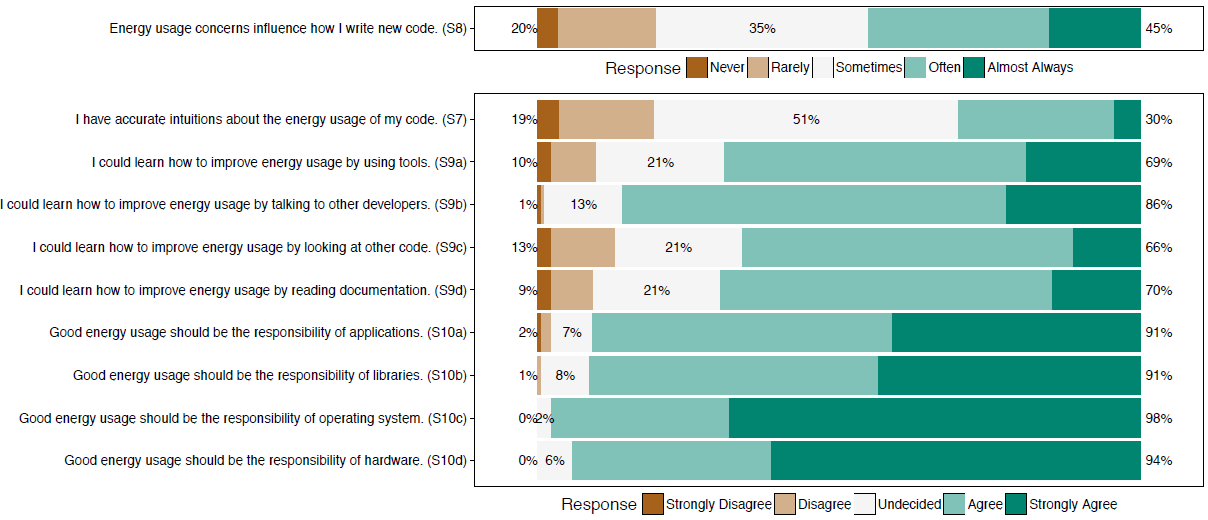
\includegraphics[width=1\textwidth]{MemoireMaster-NestorSkoczylas/figures/Déclarations et réponses des praticiens expérimentés liées à la construction.png}
    \caption{Déclarations et réponses des praticiens expérimentés liées à la construction}
    \label{fig:declaration-reponses-praticien}
\end{figure}

Certains utilisateurs, comme le souligne l'étude~\cite{EmpiricalStudy}, estiment que \emph{« Good energy usage should be the responsibility of applications »}. Cependant, il est crucial de reconnaître que cette responsabilité est partagée, comme le montre la figure \ref{fig:declaration-reponses-praticien}. Cette figure montre que les praticiens expérimentés reconnaissent la responsabilité partagée dans l'utilisation durable des logiciels, tout en soulignant l'importance de la documentation et des outils pour les aider à améliorer leur consommation d'énergie.


Comme le souligne l'étude~\cite{SafetySecuritySustainability}, \emph{« Software engineers can contribute to sustainability by designing software systems that minimize indirect impacts and by educating users about the impacts of their actions. »} . Cela implique :

\begin{itemize}
    \item \textbf{Une conception logicielle efficace :} Choisir des technologies économes en énergie, optimiser les performances du code et minimiser la consommation de ressources.
    \item \textbf{L'optimisation des logiciels :} Mettre à jour régulièrement les logiciels pour bénéficier des dernières optimisations et corriger les bugs qui peuvent affecter la consommation d'énergie.
    \item \textbf{La formation des utilisateurs :} Sensibiliser les utilisateurs aux enjeux de la durabilité logicielle et leur fournir les outils nécessaires pour adopter des pratiques durables.
\end{itemize}


En adoptant des pratiques éclairées et en comprenant l'impact de leurs actions, les utilisateurs peuvent également jouer un rôle crucial dans la durabilité logicielle. Cela implique :

\begin{itemize}
    \item \textbf{Une utilisation responsable des logiciels :} Réduire l'utilisation inutile des logiciels, fermer les programmes lorsqu'ils ne sont pas utilisés et privilégier les solutions logicielles économes en énergie.
    \item \textbf{Comprendre l'impact de ses actions :} Savoir comment les choix de logiciels et les actions quotidiennes peuvent affecter la consommation d'énergie et l'empreinte environnementale.
    \item \textbf{Tirer parti des ressources pédagogiques :} Exploiter la documentation, les tutoriels et les guides mis à disposition par les développeurs pour apprendre à utiliser les logiciels de manière durable.
\end{itemize}


L'intégration de la durabilité environnementale en tant qu'exigence non fonctionnelle est essentielle pour une mise en œuvre réussie. Cette notion est soulignée dans~\cite{SafetySecuritySustainability}, qui stipule que : \emph{« To support the transition to sustainability, environmental sustainability must be explicitly considered as a nonfunctional requirement in the software engineering process. »} Il est crucial de formaliser les considérations de durabilité dans le cycle de vie du développement logiciel. Cela implique de les intégrer dès les phases initiales de conception et de les maintenir tout au long du processus de développement, y compris la phase de test et de déploiement.


L'étude publiée dans~\cite{ImpactGreenFeedback} identifie une lacune cruciale : \emph{« Green feedback helps in raising awareness, but users lack the knowledge and tools to apply software behavioral changes. »} Il ne suffit pas de fournir aux utilisateurs des commentaires sur l'impact environnemental de leurs choix. Pour combler le fossé entre la sensibilisation et l'action, les développeurs et autres parties prenantes doivent s'engager à :

\begin{itemize}
    \item Développer des outils conviviaux qui permettent aux utilisateurs de suivre leur utilisation de logiciels, de comprendre son impact environnemental et de faire des choix éclairés.
    \item Organiser des campagnes continues d'éducation et de sensibilisation qui dotent les utilisateurs des connaissances et des compétences nécessaires pour contribuer à une utilisation durable des logiciels.
\end{itemize}


La communauté du développement de logiciels a un rôle crucial à jouer dans la construction d'un avenir numérique durable. En adoptant une approche collaborative et proactive, nous pouvons transformer l'ingénierie logicielle verte en une force positive pour l'environnement.

% Responsabilité partagée et sensibilisation des utilisateurs
%~\cite{EmpiricalStudy} "Energy usage should be a shared responsibility."
%~\cite{EmpiricalStudy} "I could learn how to improve energy usage by reading documentation."
%~\cite{EmpiricalStudy} "Good energy usage should be the responsibility of applications."
%~\cite{SafetySecuritySustainability} "To support the transition to sustainability, environmental sustainability must be explicitly considered as a nonfunctional requirement in the software engineering process."
%~\cite{SafetySecuritySustainability} "Software engineers can contribute to sustainability by designing software systems that minimize indirect impacts and by educating users about the impacts of their actions."
%~\cite{ImpactGreenFeedback} "Green feedback helps in raising awareness, but users lack the knowledge and tools to apply software behavioral changes."

\subsection{Formation des utilisateurs et retour d'information}
L'éducation et l'implication des utilisateurs sont des piliers fondamentaux pour une utilisation responsable et durable des logiciels. En effet, leur compréhension des enjeux environnementaux et de leur rôle crucial dans l'adoption de pratiques durables est essentielle.


L'écoute des besoins et des attentes des utilisateurs est tout aussi importante. Comme le souligne l'étude~\cite{EmpiricalStudy}, les utilisateurs expriment un réel désir d'apprendre et de s'améliorer : \emph{« I could learn how to improve energy usage by reading documentation. »} La figure \ref{fig:declaration-reponses-praticien} montre que 70\% des praticiens expérimentés estiment que la documentation peut les aider à améliorer leur consommation d'énergie. Cela confirme le besoin crucial de ressources éducatives accessibles et attractives pour répondre à la demande des utilisateurs.Répondre à cette demande par des ressources éducatives accessibles et attractives est donc un enjeu majeur. Cela passe par la création de :

\begin{itemize}
    \item Documentations claires et concises qui exposent l'impact environnemental des logiciels et proposent des solutions concrètes pour l'optimiser.
    \item Tutoriels interactifs et campagnes de sensibilisation qui engagent les utilisateurs et transmettent de manière ludique l'importance de pratiques durables.
\end{itemize}

En outre, responsabiliser les utilisateurs en leur offrant les connaissances et les outils nécessaires est crucial. Comme le souligne~\cite{SafetySecuritySustainability}, \emph{« Software engineers can contribute to sustainability by [...] educating users about the impacts of their actions. »} En dotant les utilisateurs de moyens d'action concrets, nous leur permettons de participer activement à la construction d'un écosystème logiciel durable.


L'étude de~\cite{ImpactGreenFeedback} souligne l'importance de \emph{« Green feedback helps in raising awareness »}. Cependant, elle met également en lumière ses limites :
\begin{itemize}
    \item \textbf{Manque de connaissances et d'outils :} \emph{« Users lack the knowledge and tools to apply software behavioral changes. »} Fournir des commentaires ne suffit pas nécessairement à engendrer des changements significatifs.
    \item \textbf{Intrusion et surcharge d'informations :} \emph{« Green feedback tools must be minimal and seamlessly integrated to avoid being distracted. »} Les mécanismes de feedback doivent être centrés sur l'utilisateur, non intrusifs et fournir des informations exploitables pour responsabiliser les utilisateurs sans les submerger.
\end{itemize}


Pour dépasser ces limites, il est essentiel de repenser la rétroaction verte. Voici quelques pistes d'amélioration :
\begin{itemize}
    \item Développez des outils conviviaux qui suivent l’utilisation des logiciels, visualisent leur impact environnemental et proposent des suggestions d’optimisation.
    \item Intégrez des mécanismes de feedback de manière transparente dans l'interface du logiciel pour minimiser les distractions et encourager l'engagement des utilisateurs.
    \item Fournissez des informations claires et exploitables grâce à des commentaires pour aider les utilisateurs à comprendre l'impact de leurs choix et à prendre des décisions éclairées concernant leur utilisation du logiciel.
\end{itemize}


L'éducation et la rétroaction efficace des utilisateurs constituent les piliers d'un avenir numérique durable. En comblant le déficit de connaissances et en responsabilisant les utilisateurs, nous pouvons construire un écosystème logiciel plus collaboratif et respectueux de l'environnement.


L'éducation permet aux utilisateurs de comprendre l'impact environnemental de leurs choix. Des ressources éducatives accessibles et attractives, telles que des tutoriels interactifs et des campagnes de sensibilisation, peuvent les aider à adopter des pratiques logicielles durables.


La rétroaction efficace fournit aux utilisateurs des informations exploitables sur leur consommation d'énergie. Des outils conviviaux qui suivent l'utilisation des logiciels, visualisent l'impact environnemental et proposent des suggestions d'optimisation peuvent les inciter à agir de manière responsable.


En combinant ces deux approches, nous pouvons créer un cercle vertueux. Les utilisateurs informés et responsabilisés peuvent influencer les développeurs, les incitant à concevoir des logiciels plus économes en énergie et à intégrer la durabilité comme une exigence fondamentale.

% Formation des utilisateurs et retour d'information
%~\cite{EmpiricalStudy} "I could learn how to improve energy usage by reading documentation."
%~\cite{SafetySecuritySustainability} "Software engineers can contribute to sustainability by designing software systems that minimize indirect impacts and by educating users about the impacts of their actions."
%~\cite{ImpactGreenFeedback} "Green feedback helps in raising awareness, but users lack the knowledge and tools to apply software behavioral changes."
%~\cite{ImpactGreenFeedback} "Green feedback tools must be minimal and seamlessly integrated to avoid being distracted."

\subsection{Concevoir pour un comportement durable}
La conception de logiciels durables ne se limite pas à l'optimisation technique. Elle vise également à influencer le comportement des utilisateurs vers des pratiques plus responsables et respectueuses de l'environnement.


L'étude de~\cite{SafetySecuritySustainability} met en lumière une perspective intéressante : \emph{« If sustainability policies and standards are put in place and software engineers prioritize them in the systems they develop, future technology may significantly contribute indirectly to influencing the behavior of users who interact with those systems in some ways while directly contributing to saving the planet. »} Ce passage souligne le pouvoir des logiciels bien conçus d'inciter les utilisateurs à adopter des comportements plus durables. En intégrant des fonctionnalités et des caractéristiques orientées vers la durabilité, les logiciels peuvent aller au-delà de leur simple fonction et devenir de véritables catalyseurs de changement.


Comment les logiciels peuvent-ils influencer les utilisateurs ?


Plusieurs leviers de conception peuvent être utilisés pour encourager les pratiques éco-responsables :

\begin{itemize}
    \item \textbf{Transparence et feedback écologique :} Informer les utilisateurs sur l'impact environnemental de leurs actions et de l'utilisation du logiciel les sensibilise et les incite à faire des choix plus informés.
    \item \textbf{Nudges et architecture de choix :} Des suggestions subtiles et une organisation réfléchie de l'interface peuvent guider les utilisateurs vers des options plus éco-responsables, sans pour autant limiter leur liberté de choix.
    \item \textbf{Gamification et motivation :} L'intégration d'éléments ludiques, comme des points et des classements, peut rendre l'utilisation durable du logiciel plus attrayante et motivante.
    \item \textbf{Par défaut durable :} Définir des options par défaut éco-responsables peut inciter les utilisateurs à adopter ces pratiques sans effort supplémentaire.
\end{itemize}


L'article~\cite{SafetySecuritySustainability} met en exergue l'importance cruciale de formaliser la prise en compte de la durabilité dans le développement logiciel. Il affirme : \emph{« To support the transition to sustainability, environmental sustainability must be explicitly considered as a nonfunctional requirement in the software engineering process. »} En d'autres termes, la durabilité ne doit pas être reléguée au second plan, mais bel et bien s'ériger comme une exigence fondamentale au même titre que la sécurité, la performance ou la maintenabilité.


L'article~\cite{SafetySecuritySustainability} rappelle le rôle crucial des ingénieurs logiciels dans la promotion de la durabilité : \emph{« Software engineers can contribute to sustainability by designing software systems that minimize indirect impacts and by educating users about the impacts of their actions. »} Leur influence sur le comportement des utilisateurs se manifeste à travers plusieurs leviers :
\begin{itemize}
    \item \textbf{Conception de fonctionnalités durables :} Intégrer des options favorisant l'efficacité des ressources et décourageant le gaspillage permet d'agir directement sur l'impact environnemental du logiciel.
    \item \textbf{Feedback écologique transparent :} Fournir des informations claires et accessibles au sein du logiciel sensibilise les utilisateurs aux implications de leurs choix et encourage des pratiques plus responsables.
    \item \textbf{Optimisation énergétique intrinsèque :} Comme le souligne~\cite{GreenMeasurementStructure}, \emph{« The software can minimise power consumption by being more energy-efficient (i.e., by becoming greener); utilizing lesser power or adopting more sustainable and supported procedures will diminish the environmental effects of software used by governments, organizations, and people. »} L’importance de concevoir des logiciels intrinsèquement économes en énergie, réduisent dès le départ leur empreinte environnementale.
\end{itemize}


La communauté des développeurs de logiciels possède un pouvoir unique : créer des logiciels qui minimisent leur propre impact environnemental tout en influençant positivement le comportement des utilisateurs. Cette double approche est essentielle pour construire un avenir numérique plus durable.


Concevoir des logiciels durables ne se résume pas à une simple optimisation technique. Il s'agit d'une démarche holistique qui prend en compte l'ensemble du cycle de vie du logiciel et intègre la durabilité comme une exigence fondamentale.

% Concevoir pour un comportement durable
%~\cite{SafetySecuritySustainability} "If sustainability policies and standards are put in place and software engineers prioritize them in the systems they develop, future technology may significantly contribute indirectly to influencing the behavior of users who interact with those systems in some ways while directly contributing to saving the planet."
%~\cite{SafetySecuritySustainability} "To support the transition to sustainability, environmental sustainability must be explicitly considered as a nonfunctional requirement in the software engineering process."
%~\cite{SafetySecuritySustainability} "Software engineers can contribute to sustainability by designing software systems that minimize indirect impacts and by educating users about the impacts of their actions."
%~\cite{GreenMeasurementStructure} "The software can minimise power consumption by being more energy-efficient (i.e., by becoming greener); utilizing lesser power or adopting more sustainable and supported procedures will diminish the environmental effects of software used by governments, organizations, and people."

\paragraph{}
Le développement durable des logiciels ne se limite pas aux efforts des développeurs. Les utilisateurs jouent un rôle crucial en adoptant des pratiques responsables et en contribuant à l'utilisation efficace et écologique des logiciels. 
Cette section explore les moyens de promouvoir un comportement durable chez les utilisateurs, en s'attaquant aux aspects clés de la sensibilisation, de la formation et de la conception logicielle.


Sensibilisation et responsabilisation des utilisateurs :
\begin{itemize}
    \item Responsabilité partagée : La durabilité logicielle est un effort collectif. Développeurs, utilisateurs et parties prenantes doivent collaborer pour minimiser l'impact environnemental des logiciels.
    \item Sensibilisation et éducation : Fournir aux utilisateurs des ressources accessibles et compréhensibles pour les sensibiliser aux implications énergétiques de leurs actions et les inciter à adopter des pratiques durables.
    \item Outils et information : Développer des outils conviviaux qui permettent aux utilisateurs de suivre leur utilisation des logiciels et de comprendre son impact environnemental.
    \item Campagnes de sensibilisation : Organiser des campagnes continues pour diffuser des informations sur l'importance des pratiques logicielles durables et responsabiliser les utilisateurs.
\end{itemize}


Formation et responsabilisation des utilisateurs :
\begin{itemize}
    \item Combler le déficit de connaissances : Fournir aux utilisateurs des ressources éducatives facilement accessibles, telles que des tutoriels, des guides et des formations, pour leur donner les compétences nécessaires pour contribuer à la durabilité logicielle.
    \item Feedback efficace : Concevoir des mécanismes de feedback non intrusifs et exploitables qui intègrent des suggestions d'optimisation et des informations claires sur l'impact environnemental des choix des utilisateurs.
    \item Autonomisation des utilisateurs : Donner aux utilisateurs les moyens de prendre des décisions éclairées en matière d'utilisation des logiciels en leur fournissant des informations et des outils pertinents.
\end{itemize}


Concevoir pour un comportement durable :
\begin{itemize}
    \item Intentionnalité et influence : Concevoir des logiciels qui incitent les utilisateurs à adopter des pratiques plus responsables et respectueuses de l'environnement.
    \item Fonctionnalités durables : Intégrer des fonctionnalités qui favorisent l'efficacité des ressources et découragent le gaspillage.
    \item Information accessible : Fournir des informations claires et contextuelles au sein du logiciel sur l'impact environnemental des actions des utilisateurs.
    \item Optimisation de l'efficacité : Concevoir des logiciels intrinsèquement économes en énergie pour réduire leur empreinte environnementale dès le départ.
\end{itemize}


En sensibilisant, en formant et en responsabilisant les utilisateurs, et en concevant des logiciels qui encouragent des pratiques durables, la communauté des développeurs de logiciels peut créer un avenir plus vert et plus durable. La collaboration et l'engagement de tous les acteurs sont essentiels pour réaliser cet objectif.

%%%%%%%%%%%%%%%%%%%%%%%%%%%%%%%%%%%%

\paragraph{Conclusion}
Ce chapitre a exploré l'influence cruciale des pratiques individuelles des développeurs sur la durabilité des logiciels. Au-delà des aspects techniques, il a mis en lumière l'importance de la responsabilité individuelle et de l'engagement dans la création d'un avenir numérique plus vert.


Que faut-il retenir de ce chapitre ?
\begin{enumerate}
    \item Sensibilisation et connaissances : La sensibilisation aux impacts environnementaux du développement logiciel est le point de départ. Les développeurs doivent acquérir les connaissances nécessaires pour prendre des décisions éclairées et adopter des pratiques durables.
    \item Engagement et responsabilité : Chaque développeur est responsable de l'empreinte environnementale de son code. Adopter une attitude pro-active et responsable est crucial pour contribuer à un avenir plus durable.
    \item Pratiques et outils durables : De nombreuses pratiques et outils existent pour aider les développeurs à réduire l'impact environnemental de leur travail. Il est important de les connaître et de les utiliser de manière optimale.
    \item Collaboration et partage des connaissances : La collaboration entre les développeurs, les équipes et les organisations est essentielle pour faire progresser les pratiques durables dans l'industrie du logiciel.
    \item Mesure et évaluation : Suivre et évaluer l'impact environnemental des logiciels est crucial pour identifier les domaines d'amélioration et mesurer les progrès accomplis.
    \item Engagement continu : La durabilité logicielle n'est pas une destination finale, mais un voyage continu. Il est important de rester engagé et de s'adapter aux nouvelles technologies et aux meilleures pratiques émergentes.
\end{enumerate}


En résumé, les développeurs ont le pouvoir de jouer un rôle crucial dans la création d'un avenir numérique plus durable. 
En adoptant une conscience accrue, en s'engageant à des pratiques responsables et en collaborant avec la communauté, ils peuvent contribuer à un changement positif et significatif.

\paragraph{Transition vers Intégration de la Durabilité à Différentes Échelles dans le Développement Logiciel}
Le deuxième chapitre a mis en lumière l'importance des pratiques individuelles des développeurs dans la construction de logiciels durables. Nous avons conclu en soulignant la nécessité d'une responsabilité individuelle et d'un engagement continu pour un avenir numérique plus écologique.


Or, la durabilité logicielle ne se limite pas aux actions individuelles. Elle exige une approche globale qui intègre des pratiques durables à différentes échelles, allant des projets et des équipes de développement jusqu'à la stratégie d'entreprise. C'est précisément l'objet du \ref{pratique-globale}, qui explore comment intégrer la durabilité à différentes échelles dans le développement logiciel.


Ce chapitre examinera comment les projets logiciels peuvent être planifiés et exécutés en tenant compte de la durabilité. Il se penchera également sur les pratiques durables au niveau des équipes de développement et sur la manière dont les entreprises peuvent aligner leur stratégie sur les objectifs de durabilité logicielle.


En explorant ces différentes échelles d'action, le \ref{pratique-globale} vise à démontrer l'importance d'une approche multidimensionnelle pour un développement logiciel véritablement durable.
